% Lumped mass model of the webbing: overview of the chain and a zoom on node i.
% Build:  pdflatex spring_chain.tex && pdftops -eps spring_chain.pdf spring_chain.eps
\documentclass[tikz,border=4pt]{standalone}
\usetikzlibrary{decorations.pathmorphing,patterns,arrows.meta,calc}

\begin{document}
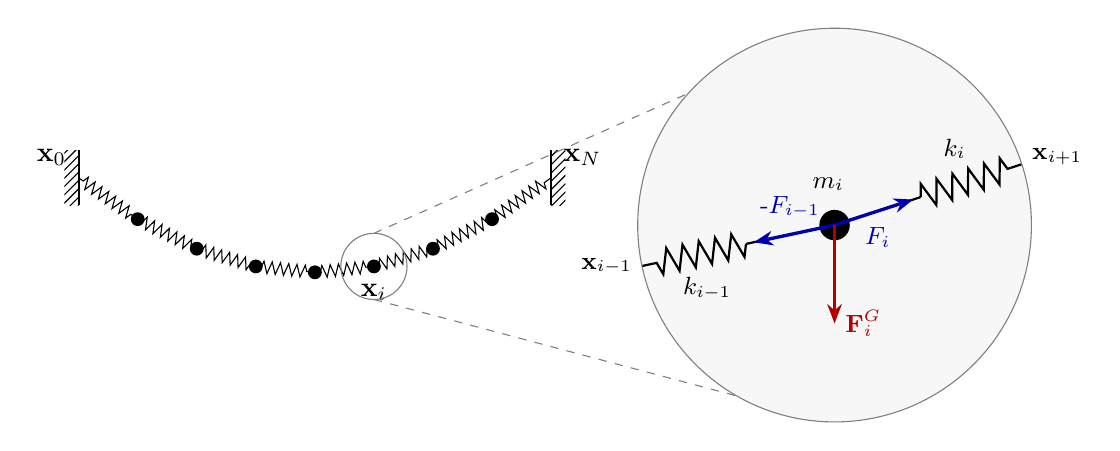
\begin{tikzpicture}[
    mass/.style={circle,fill=black,inner sep=0pt,minimum size=5pt},
    bigmass/.style={circle,fill=black,inner sep=0pt,minimum size=11pt},
    spring/.style={decorate,decoration={zigzag,segment length=3pt,amplitude=2.2pt,
                   pre length=2pt,post length=2pt}},
    bigspring/.style={decorate,decoration={zigzag,segment length=6pt,amplitude=4.5pt}},
    force/.style={-{Stealth[length=7pt]},very thick},
    zoomline/.style={gray,dashed,thin},
  ]

  % ---------------------------------------------------------------- overview
  % Parabolic sag, y = -s (1 - ((x - 3)/3)^2), N = 8 edges
  \def\s{1.2}
  \foreach \j in {0,...,8} {
    \pgfmathsetmacro{\x}{0.75*\j}
    \pgfmathsetmacro{\y}{-\s*(1-((\x-3)/3)^2)}
    \coordinate (n\j) at (\x,\y);
  }
  \foreach \j [evaluate=\j as \jn using int(\j+1)] in {0,...,7}
    \draw[spring] (n\j) -- (n\jn);
  \foreach \j in {1,...,7} \node[mass] at (n\j) {};

  % Fixed anchors
  \foreach \a/\d in {n0/-1, n8/1} {
    \fill[pattern=north east lines] ($(\a)+(0,-0.35)$) rectangle ($(\a)+(0.18*\d,0.35)$);
    \draw[thick] ($(\a)+(0,-0.35)$) -- ($(\a)+(0,0.35)$);
  }
  \node[above left=1pt]  at (n0) {$\mathbf{x}_0$};
  \node[above right=1pt] at (n8) {$\mathbf{x}_N$};
  \node[below=3pt]       at (n5) {$\mathbf{x}_i$};

  % ---------------------------------------------------------------- zoom
  \def\r{0.42}   % radius of the small circle
  \def\R{2.5}    % radius of the zoom panel
  \coordinate (Z) at (9.6,-0.6);
  \draw[gray] (n5) circle (\r);
  \draw[zoomline] ($(n5)+(0,\r)$)  -- ($(Z)+(0,\R)$);
  \draw[zoomline] ($(n5)+(0,-\r)$) -- ($(Z)+(0,-\R)$);

  \begin{scope}
    \clip (Z) circle (\R);
    \fill[gray!6] (Z) circle (\R);

    % One edge: a lead, then a spring, then a lead.
    % #1 = angle of the edge, #2 = label of its spring
    \newcommand{\kedge}[2]{
      \begin{scope}[shift={(Z)},rotate=#1]
        \draw[thick] (0,0) -- (1.15,0);
        \draw[thick,bigspring] (1.15,0) -- (2.35,0);
        \draw[thick] (2.35,0) -- (3.2,0);
        \node[font=\small] at (1.75,0.45) {#2};
      \end{scope}
    }
    \kedge{192}{$k_{i-1}$}
    \kedge{18}{$k_{i}$}
  \end{scope}
  \draw[gray] (Z) circle (\R);

  % Forces on node i
  \node[bigmass] (m) at (Z) {};
  \node[font=\small] at ($(Z)+(-0.08,0.52)$) {$m_i$};
  \draw[force,blue!70!black] (Z) -- ++(192:1.05)
    node[pos=0.55,above=2pt,font=\small] {-$F_{i-1}$};
  \draw[force,blue!70!black] (Z) -- ++(18:1.05)
    node[pos=0.55,below=2pt,font=\small] {$F_{i}$};
  \draw[force,red!70!black] (Z) -- ++(0,-1.25)
    node[right,font=\small] {$\mathbf{F}_i^G$};

  % Neighbour labels outside the panel
  \node[font=\small] at ($(Z)+(192:\R)+(-0.45,0)$) {$\mathbf{x}_{i-1}$};
  \node[font=\small] at ($(Z)+(18:\R)+(0.45,0.1)$) {$\mathbf{x}_{i+1}$};
\end{tikzpicture}
\end{document}
